% \documentclass[handout]{beamer}
\documentclass{beamer}

\mode<presentation>
{
  \usetheme{ANLBlue}
  % \usefonttheme[onlymath]{serif}
  % \usetheme{Singapore}
  % \usetheme{Warsaw}
  % \usetheme{Malmoe}
  % \useinnertheme{circles}
  % \useoutertheme{infolines}
  % \useinnertheme{rounded}

  \setbeamercovered{transparent=20}
}

\usepackage[english]{babel}
\usepackage[latin1]{inputenc}
\usepackage{alltt,listings,multirow,ulem,siunitx}
\usepackage[absolute,overlay]{textpos}
\TPGrid{1}{1}
\usepackage{pdfpages}
\usepackage{ulem}
\usepackage{multimedia}
\usepackage{multicol}
\newcommand\hmmax{0}
\newcommand\bmmax{0}
\usepackage{bm}
\usepackage{comment}

% font definitions, try \usepackage{ae} instead of the following
% three lines if you don't like this look
\usepackage{mathptmx}
\usepackage[scaled=.90]{helvet}
% \usepackage{courier}
\usepackage[T1]{fontenc}
\usepackage{tikz}
\usetikzlibrary{decorations.pathreplacing}
\usetikzlibrary{shadows,arrows,shapes.misc,shapes.arrows,shapes.multipart,arrows,decorations.pathmorphing,backgrounds,positioning,fit,petri,calc,shadows,chains,matrix}

\newcommand\vvec{\bm v}
\newcommand\bvec{\bm b}
\newcommand\bxk{\bvec_0 \times \kappa_0 \cdot \nabla}
\newcommand\delp{\nabla_\perp}

% \usepackage{pgfpages}
% \pgfpagesuselayout{4 on 1}[a4paper,landscape,border shrink=5mm]

\usepackage{JedMacros}

\newcommand{\timeR}{t_{\mathrm{R}}}
\newcommand{\timeW}{t_{\mathrm{W}}}
\newcommand{\mglevel}{\ensuremath{\ell}}
\newcommand{\mglevelcp}{\ensuremath{\mglevel_{\mathrm{cp}}}}
\newcommand{\mglevelcoarse}{\ensuremath{\mglevel_{\mathrm{coarse}}}}
\newcommand{\mglevelfine}{\ensuremath{\mglevel_{\mathrm{fine}}}}

%solution and residual
\newcommand{\vx}{\ensuremath{x}}
\newcommand{\vc}{\ensuremath{\hat{x}}}
\newcommand{\vr}{\ensuremath{r}}
\newcommand{\vb}{\ensuremath{b}}

%operators
\newcommand{\vA}{\ensuremath{A}}
\newcommand{\vP}{\ensuremath{I_H^h}}
\newcommand{\vS}{\ensuremath{S}}
\newcommand{\vR}{\ensuremath{I_h^H}}
\newcommand{\vI}{\ensuremath{\hat I_h^H}}
\newcommand{\vV}{\ensuremath{\mathbf{V}}}
\newcommand{\vF}{\ensuremath{F}}
\newcommand{\vtau}{\ensuremath{\mathbf{\tau}}}


\title{Prospects for next-generation multigridding}
\subtitle{low communication, low memory, adaptive, \\ composable, and resilient}
\author{{\bf Jed Brown} \\
Mark Adams, Peter Brune, Emil Constantinescu, \\
Matt Knepley, Dave May, Barry Smith \\
\texttt{jedbrown@mcs.anl.gov}
}

% - Use the \inst command only if there are several affiliations.
% - Keep it simple, no one is interested in your street address.
\institute
{
  Mathematics and Computer Science Division \\ Argonne National Laboratory
}

\date{Oxford, 2013-09-27}

% This is only inserted into the PDF information catalog. Can be left
% out.
\subject{Talks}


% If you have a file called "university-logo-filename.xxx", where xxx
% is a graphic format that can be processed by latex or pdflatex,
% resp., then you can add a logo as follows:

% \pgfdeclareimage[height=0.5cm]{university-logo}{university-logo-filename}
% \logo{\pgfuseimage{university-logo}}



% Delete this, if you do not want the table of contents to pop up at
% the beginning of each subsection:
% \AtBeginSubsection[]
% {
% \begin{frame}<beamer>
%   \frametitle{Outline}
%   \tableofcontents[currentsection,currentsubsection]
% \end{frame}
% }

\AtBeginSection[]
{
  \begin{frame}<beamer>
    \frametitle{Outline}
    \tableofcontents[currentsection]
  \end{frame}
}

% If you wish to uncover everything in a step-wise fashion, uncomment
% the following command:

% \beamerdefaultoverlayspecification{<+->}

\begin{document}
\lstset{language=C}
\normalem

\begin{frame}
  \titlepage
\end{frame}

\section{Hardware/algorithm tradeoffs}
\begin{frame}{Bottlenecks of (Jacobian-free) Newton-Krylov}
  \begin{columns}
    \begin{column}{0.4\textwidth}
      \includegraphics[width=1.15\textwidth]{figures/Dohp/EllipRCM}
    \end{column}
    \begin{column}{0.6\textwidth}
      \begin{itemize}
      \item Matrix assembly
        \begin{itemize}
        \item integration/fluxes: FPU
        \item insertion: memory/branching
        \end{itemize}
      \item Preconditioner setup
        \begin{itemize}
        \item coarse level operators
        \item overlapping subdomains
        \item (incomplete) factorization
        \end{itemize}
      \item Preconditioner application
        \begin{itemize}
        \item triangular solves/relaxation: memory
        \item coarse levels: network latency
        \end{itemize}
      \item Matrix multiplication
        \begin{itemize}
        \item Sparse storage: memory
        \item Matrix-free: FPU
        \end{itemize}
      \item Globalization
      \end{itemize}
    \end{column}
  \end{columns}
\end{frame}

\begin{frame}{Scalability Warning}
  \begin{quote}\Large \centering
    The easiest way to make software scalable \\
    is to make it sequentially inefficient. \\
    (Gropp 1999)
  \end{quote}

  \begin{itemize}
  \item We really want \emph{efficient} software
  \item Need a performance model
    \begin{itemize}
    \item memory bandwidth and latency
    \item algorithmically critical operations (\eg dot products, scatters)
    \item floating point unit
    \end{itemize}
  \item Scalability shows marginal benefit of adding more cores, nothing more
  \item Constants hidden in the choice of algorithm
  \item Constants hidden in implementation
  \end{itemize}
\end{frame}

\begin{frame}{Hardware Arithmetic Intensity}
  \begin{tabular}{lc}
    \toprule
    Operation                         & Arithmetic Intensity (flops/B) \\
    \midrule
    Sparse matrix-vector product      & 1/6                  \\
    Dense matrix-vector product       & 1/4                  \\
    Unassembled matrix-vector product & $\approx 8$          \\
    High-order residual evaluation    & $> 5$                \\
    \bottomrule
  \end{tabular}

  \bigskip

  \begin{tabular}{lrrr}
    \toprule
    Processor & BW (GB/s) & Peak (GF/s) & Balanced AI (F/B) \\
    \midrule
    E5-2670 8-core      & 35   & 166  & 4.7 \\
    Magny Cours 16-core & 49   & 281  & 5.7 \\
    Blue Gene/Q node    & 43   & 205  & 4.8 \\
    Tesla M2090         & 120  & 665  & 5.5 \\
    Kepler K20Xm        & 160 & 1310 & 8.2 \\ % http://www.elekslabs.com/2012/11/nvidia-tesla-k20-benchmark-facts.html
    Xeon Phi            & 150 & 1248 & 8.3 \\
    \bottomrule
  \end{tabular}
\end{frame}

\begin{frame}[shrink=5]{Performance of assembled versus unassembled}
  \vspace{1ex}
  \includegraphics[width=\textwidth]{figures/TensorVsAssembly} \\
  \begin{itemize}
  \item Arithmetic intensity for $\Qk p$ elements
    \begin{itemize}
    \item $< \frac 1 4$ (assembled), $\approx 10$ (unassembled), $\approx 4$ to $8$ (hardware)
    \end{itemize}
  \item store Jacobian information at Quass quadrature points, can use AD
  \end{itemize}
\end{frame}

\begin{frame}{\texttt{MPI\_Allreduce} performance, c/o Paul Fischer}
  \includegraphics[width=\textwidth]{figures/hardware/FischerBGQAllReduce.png}
\end{frame}
\begin{frame}{Packaging versus efficiency}
  \includegraphics[width=\textwidth]{figures/hardware/MKL-dgeqrf-MIC.png}
  \begin{itemize}
  \item 1 MIC (Xeon Phi): 300 W TDP and \$4200
  \item 1 Xeon: 115 W TDP and \$1300
  \end{itemize}
\end{frame}

\section{Multigrid}
\begin{frame}[fragile]{Multigrid Preliminaries}
  \begin{figure}
    \centering
    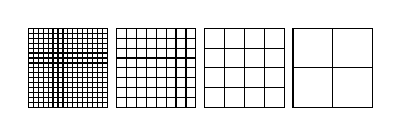
\begin{tikzpicture}
      [>=stealth,
      every node/.style={inner sep=2pt},
      restrict/.style={thick},
      prolong/.style={thick},
      mglevel/.style={rounded rectangle,draw=blue!50!black,fill=blue!20,thick,minimum size=4mm},
      ]
      \begin{scope}\scriptsize
        \newcommand\mgdx{4.0em}
        \newcommand\mgdy{4.0em}
        \newcommand\mgl[1]{(pow(2,#1+1))}
        \newcommand\mgloc[4]{(#1 + #4*\mgdx*#3,#2 + \mgdy*#3)}

        \newcommand\mghx{0.9*\mgdx}
        \newcommand\mghy{0.9*\mgdy}

        \draw[shift=\mgloc{0*\mgdx}{0}{0}{0},
        xstep=\mghy/\mgl{3},
        ystep=\mghy/\mgl{3}]
        (-0.5*\mghy,-0.5*\mghy) grid (0.5*\mghy,0.5*\mghy);

        \draw[shift=\mgloc{1*\mgdx}{0}{0}{0},
        xstep=\mghy/\mgl{2},
        ystep=\mghy/\mgl{2}]
        (-0.5*\mghy,-0.5*\mghy) grid (0.5*\mghy,0.5*\mghy);

        \draw[shift=\mgloc{2*\mgdx}{0}{0}{0},
        xstep=\mghy/\mgl{1},
        ystep=\mghy/\mgl{1}]
        (-0.5*\mghy,-0.5*\mghy) grid (0.5*\mghy,0.5*\mghy);


        \draw[shift=\mgloc{3*\mgdx}{0}{0}{0},
        xstep=\mghy/\mgl{0},
        ystep=\mghy/\mgl{0}]
        (-0.5*\mghy,-0.5*\mghy) grid (0.5*\mghy,0.5*\mghy);
      \end{scope}
    \end{tikzpicture}
    \label{fig:levels}
  \end{figure}
  \textbf{Multigrid} is an $O(n)$ method for solving algebraic problems by defining a hierarchy of scale.
  A multigrid method is constructed from:
  \begin{enumerate}
  \item a series of discretizations
    \begin{itemize}
    \item coarser approximations of the original problem
    \item constructed algebraically or geometrically
    \end{itemize}
  \item intergrid transfer operators
    \begin{itemize}
    \item residual restriction $I_h^H$ (fine to coarse)
    \item state restriction $\hat I_h^H$ (fine to coarse)
    \item partial state interpolation $I_H^h$ (coarse to fine, `prolongation')
    \item state reconstruction $\mathbb{I}_H^h$ (coarse to fine)
    \end{itemize}
  \item Smoothers ($S$)
    \begin{itemize}
    \item correct the high frequency error components
    \item Richardson, Jacobi, Gauss-Seidel, etc.
    \item Gauss-Seidel-Newton or optimization methods
    \end{itemize}
  \end{enumerate}
\end{frame}

\begin{frame}[fragile]
  \frametitle{Multigrid}
  \begin{itemize}
    \item \textbf{Multigrid} methods uses coarse correction for large-scale error
  \end{itemize}
  \begin{figure}
  \centering
  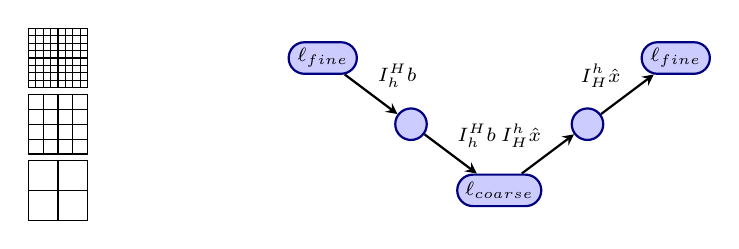
\begin{tikzpicture}
    [>=stealth,
    every node/.style={inner sep=2pt},
    restrict/.style={thick},
    prolong/.style={thick},
    mglevel/.style={rounded rectangle,draw=blue!50!black,fill=blue!20,thick,minimum size=4mm},
    ]
    \begin{scope}\scriptsize
      \newcommand\mgdx{4.0em}
      \newcommand\mgdy{3.0em}
      \newcommand\mgl[1]{(pow(2,#1+1))}
      \newcommand\mgloc[4]{(#1 + #4*\mgdx*#3,#2 + \mgdy*#3)}
      \node[mglevel] (down0) at \mgloc{0}{0}{2}{-1} {\mglevel$_{fine}$};
      \node[mglevel] (down1) at \mgloc{0}{0}{1}{-1} {};
      \node[mglevel] (coarse) at \mgloc{0}{0}{0}{-1} {\mglevel$_{coarse}$};

      \node[mglevel] (up1) at \mgloc{0}{0}{1}{1} {};
      \node[mglevel] (up0) at \mgloc{0}{0}{2}{1} {\mglevel$_{fine}$};

      \path[->,restrict] (down0) edge node [above right] {$\vR\vb$} (down1)
                         (down1) edge node [above right] {$\vR\vb$} (coarse);

      \path[->,prolong] (coarse) edge node [above left] {$\vP\vc$} (up1)
                         (up1) edge node [above left] {$\vP\vc$} (up0);

      %grids
      \newcommand\mghx{0.9*\mgdx}
      \newcommand\mghy{0.9*\mgdy}

      \draw[shift=\mgloc{-5*\mgdx}{0}{2}{0},
      xstep=\mghy/\mgl{2},
      ystep=\mghy/\mgl{2}]
      (-0.5*\mghy,-0.5*\mghy) grid (0.5*\mghy,0.5*\mghy);

      \draw[shift=\mgloc{-5*\mgdx}{0}{1}{0},
      xstep=\mghy/\mgl{1},
      ystep=\mghy/\mgl{1}]
      (-0.5*\mghy,-0.5*\mghy) grid (0.5*\mghy,0.5*\mghy);

      \draw[shift=\mgloc{-5*\mgdx}{0}{0}{0},
      xstep=\mghy/\mgl{0},
      ystep=\mghy/\mgl{0}]
      (-0.5*\mghy,-0.5*\mghy) grid (0.5*\mghy,0.5*\mghy);

  \end{scope}
\end{tikzpicture}
\label{fig:MG}
\end{figure}
Algorithm $MG(\vA,\vb)$ for the solution of $\vA\vx = \vb$:
\begin{align*}
  &\vx = \vS^m(\vx,\vb)             & \text{pre-smooth}\\
  &\vb^{H} = \vR(\vr - \vA\vx)       & \text{restrict residual}\\
  &\vc^{H} = MG(\vR\vA\vP,\vb^{H})   & \text{recurse}\\
  &\vx = \vx + \vP\vc^{H}            & \text{prolong correction}\\
  &\vx = \vx + \vS^n(\vx,\vb)       & \text{post-smooth}\\
\end{align*}
\end{frame}

\begin{frame}[fragile]
  \frametitle{Full Multigrid(FMG)}
  \begin{figure}
  \centering
  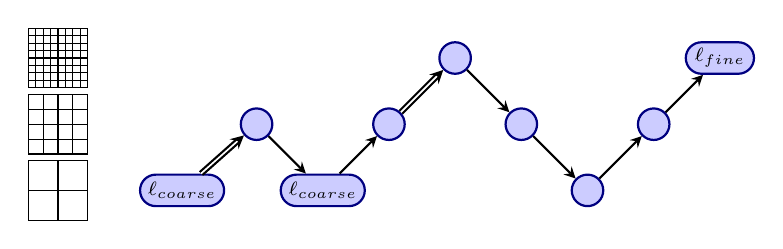
\begin{tikzpicture}
    [>=stealth,
    every node/.style={inner sep=2pt},
    restrict/.style={thick},
    prolong/.style={thick},
    mglevel/.style={rounded rectangle,draw=blue!50!black,fill=blue!20,thick,minimum size=4mm},
    ]
    \begin{scope}\scriptsize
      \newcommand\mgdx{3.0em}
      \newcommand\mgdy{3.0em}
      \newcommand\mgl[1]{(pow(2,#1+1))}
      \newcommand\mgloc[4]{(#1 + #4*\mgdx*#3,#2 + \mgdy*#3)}

      \node[mglevel] (coarseinit) at \mgloc{-3}{0}{0}{0} {$\mglevel_{coarse}$};

      \node[mglevel] (afine) at \mgloc{0}{0}{1}{1} {};

      \node[mglevel] (bcoarse) at \mgloc{2*\mgdx}{0}{0}{1} {$\mglevel_{coarse}$};
      \node[mglevel] (bup1) at \mgloc{2*\mgdx}{0}{1}{1} {};
      \node[mglevel] (bfine) at \mgloc{2*\mgdx}{0}{2}{1} {};

      \node[mglevel] (cdown1) at \mgloc{6*\mgdx}{0}{1}{-1} {};
      \node[mglevel] (ccoarse) at \mgloc{6*\mgdx}{0}{0}{-1} {};
      \node[mglevel] (cup1) at \mgloc{6*\mgdx}{0}{1}{1} {};
      \node[mglevel] (cfine) at \mgloc{6*\mgdx}{0}{2}{1} {$\mglevel_{fine}$};


      \draw[->,restrict,double]
                         (coarseinit) -- node [above right] {} (afine);
      \draw[->,restrict]
                         (afine) -- node [above right] {} (bcoarse);
      \draw[->,restrict]
                         (bcoarse) -- node [above right] {} (bup1);
      \draw[->,restrict,double]
                         (bup1) -- node [above right] {} (bfine);
      \draw[->,restrict]
                         (bfine) -- node [above right] {} (cdown1);
      \draw[->,restrict]
                         (cdown1) -- node [above right] {} (ccoarse);
      \draw[->,restrict]
                         (ccoarse) -- node [above right] {} (cup1);
      \draw[->,restrict]
                         (cup1) -- node [above right] {} (cfine);

      %grids
      \newcommand\mghx{0.9*\mgdx}
      \newcommand\mghy{0.9*\mgdy}

      \draw[shift=\mgloc{-2*\mgdx}{0}{2}{0},
      xstep=\mghy/\mgl{2},
      ystep=\mghy/\mgl{2}]
      (-0.5*\mghy,-0.5*\mghy) grid (0.5*\mghy,0.5*\mghy);

      \draw[shift=\mgloc{-2*\mgdx}{0}{1}{0},
      xstep=\mghy/\mgl{1},
      ystep=\mghy/\mgl{1}]
      (-0.5*\mghy,-0.5*\mghy) grid (0.5*\mghy,0.5*\mghy);

      \draw[shift=\mgloc{-2*\mgdx}{0}{0}{0},
      xstep=\mghy/\mgl{0},
      ystep=\mghy/\mgl{0}]
      (-0.5*\mghy,-0.5*\mghy) grid (0.5*\mghy,0.5*\mghy);

  \end{scope}
\end{tikzpicture}
\label{fig:FMG}
\end{figure}
\begin{itemize}
  \item start wich coarse grid
  \item $\vx$ is prolonged using $\mathbb{I}_H^h$ on first visit to each finer level
  \item truncation error within one cycle
  \item about five work units for many problems
  \item highly efficient solution method
\end{itemize}
\end{frame}

\begin{frame}{$\tau$ formulation of Full Approximation Scheme (FAS)}
  \begin{itemize}
  \item classical formulation: ``coarse grid \emph{accelerates} fine grid solution''
  \item $\tau$ formulation: ``fine grid improves accuracy of coarse grid''
  \item To solve $N u = f$, recursively apply
    \begin{equation*}
      \begin{split}
        \text{pre-smooth} \:\: & \quad \tilde u^h \gets S^h_{\text{pre}}(u^h_0, f^h) \\
        \text{solve coarse problem for $u^H$} \:\: & \quad N^H u^H = f^H + \underbrace{N^H \hat I_h^H \tilde u^h - I_h^H N^h \tilde u^h}_{\tau_h^H} \\
        \text{correction and post-smooth} \:\: & \quad u^h \gets S^h_{\text{post}} \Big( \tilde u^h + I_H^h (u^H - \hat I_h^H \tilde u^h), f^h \Big) \\
      \end{split}
    \end{equation*}
    \begin{tabular}{ll}
      \toprule
      $I_h^H$ & residual restriction \\
      $\hat I_h^H$ & solution restriction \\
      $I_H^h$ & solution interpolation \\
      $f^H = I_h^H f^h$ & restriction of forcing term \\
      $\{S^h_{\text{pre}},S^h_{\text{post}}\}$ & smoothing operations on the fine grid \\
      \bottomrule
    \end{tabular}
  \end{itemize}
\end{frame}

\begin{frame}{Multiscale compression and recovery using $\tau$}
  % \begin{tikzpicture}
  %   [>=stealth,
  %   every node/.style={inner sep=2pt},
  %   restrict/.style={thick,double},
  %   prolong/.style={thick,double},
  %   cprestrict/.style={green!50!black,thick,double,dashed},
  %   control/.style={rectangle,red!40!black,draw=red!40!black,thick},
  %   mglevel/.style={rounded rectangle,draw=blue!50!black,fill=blue!20,thick,minimum size=4mm},
  %   checkpoint/.style={rectangle,draw=green!50!black,fill=green!20,thick,minimum size=4mm},
  %   mglevelhide/.style={rounded rectangle,draw=gray!50!black,fill=gray!20,thick,minimum size=4mm},
  %   tau/.style={text=red!50!black,draw=red!50!black,fill=red!10,inner sep=1pt}
  %   ]
  %   \begin{scope}\scriptsize
  %     \newcommand\mgdx{2.1em}
  %     \newcommand\mgdy{1.9em}
  %     \newcommand\mgloc[4]{(#1 + #4*\mgdx*#3,#2 + \mgdy*#3)}
  %     \node[mglevel] (fine0) at \mgloc{0}{0}{4}{-1} {\mglevelfine};
  %     \node[mglevel] (finem1down0) at \mgloc{0}{0}{3}{-1} {};
  %     \node[mglevel] (cp1down0) at \mgloc{0}{0}{2}{-1} {$\mglevelcp+1$};
  %     \node[mglevel] (cpdown0) at \mgloc{0}{0}{1}{-1} {\mglevelcp};
  %     \node[mglevel] (coarser0) at \mgloc{0}{0}{0}{0} {\ldots};

  %     \node[mglevelhide] (cpup0) at \mgloc{0}{0}{1}{1} {};
  %     \node (cp1up0) at \mgloc{0}{0}{2}{1} {};

  %     \node (cpdown1) at \mgloc{4em}{0}{1}{-1} {};
  %     \node[mglevelhide] (coarser1) at \mgloc{4em}{0}{0}{1} {\ldots};
  %     \node[mglevel] (cpup1) at \mgloc{4em}{0}{1}{1} {\mglevelcp};
  %     \node[mglevel] (cp1up1) at \mgloc{4em}{0}{2}{1} {$\mglevelcp+1$};
  %     \node[mglevel] (finem1up1) at \mgloc{4em}{0}{3}{1} {};
  %     \node[mglevel] (fine1) at \mgloc{4em}{0}{4}{1} {\mglevelfine};

  %     \draw[->,restrict,dashed] (fine0) -- (finem1down0);
  %     \draw[->,restrict] (finem1down0) -- (cp1down0);
  %     \draw[->,restrict] (cp1down0) -- (cpdown0);
  %     \draw[->,restrict,dashed] (cpdown0) -- (coarser0);
  %     \draw[->,prolong,dashed] (coarser0) -- (cpup0);
  %     \draw[->,prolong,dashed] (cpup0) -- (cp1up0);

  %     \draw[->,restrict,dashed] (cpdown1) -- (coarser1);
  %     \draw[->,prolong,dashed] (coarser1) -- (cpup1);
  %     \draw[->,prolong] (cpup1) -- (cp1up1);
  %     \draw[->,prolong] (cp1up1) -- (finem1up1);
  %     \draw[->,prolong,dashed] (finem1up1) -- (fine1);

  %     \node[checkpoint] at (4em + \mgdx*4,\mgdy) (cp) {CP};
  %     \draw[>->,cprestrict] (fine1) -- node[below,sloped] {Restrict} (cp);

  %     \node[left=\mgdx of fine0] (bnanchor) {};
  %     \node[control,fill=red!20] at (1.1*\mgdx,3*\mgdy) {Solve $F(u^n;b^n) = 0$};
  %     \node[mglevel,right=of fine1] (finedt) {next solve};
  %     \draw[->, >=stealth, control] (fine1) to[out=20,in=170] node[above] {$b^{n+1}(u^n,b^n)$} (finedt);
  %     \draw[->, >=stealth, control] (bnanchor) to[out=45,in=155] node[above] {$b^n$} (fine0);

  %     % Recovery process
  %     \begin{scope}[xshift=7*\mgdx]
  %       \node[checkpoint] (rcp) at \mgloc{0}{0}{0}{0} {CP};
  %       \node[mglevel] (r0a) at \mgloc{0}{\mgdy}{0}{0} {CR};
  %       \node[mglevel] (r1a) at \mgloc{0}{\mgdy}{1}{1} {};
  %       \node[mglevel] (r0b) at \mgloc{2*\mgdx}{\mgdy}{0}{0} {CR};
  %       \node[mglevel] (r1b) at \mgloc{2*\mgdx}{\mgdy}{1}{1} {};
  %       \node[mglevel] (r2b) at \mgloc{2*\mgdx}{\mgdy}{2}{1} {\mglevelfine};
  %       \node[mglevel] (r1c) at \mgloc{6*\mgdx}{\mgdy}{1}{-1} {};
  %       \node[mglevel] (r0d) at \mgloc{6*\mgdx}{\mgdy}{0}{0} {CR};
  %       \node[mglevel] (r1d) at \mgloc{6*\mgdx}{\mgdy}{1}{1} {};
  %       \node[mglevel] (r2d) at \mgloc{6*\mgdx}{\mgdy}{2}{1} {\mglevelfine};

  %       \draw[-,prolong,green!50!black] (rcp) -- (r0a);
  %       \draw[->,prolong] (r0a) -- (r1a);
  %       \draw[->,restrict] (r1a) -- (r0b);
  %       \draw[->,restrict] (r0b) -- (r1b);
  %       \draw[->,restrict,dashed] (r1b) -- (r2b);
  %       \draw[->,restrict,dashed] (r2b) -- (r1c);
  %       \draw[->,restrict] (r1c) -- (r0d);
  %       \draw[->,restrict] (r0d) -- (r1d);
  %       \draw[->,restrict,dashed] (r1d) -- (r2d);

  %       \foreach \smooth in {finem1down0, cp1down0, cpdown0, coarser0,
  %         cpup1, cp1up1, finem1up1,
  %         r0b,r1c,r0d,r1d} {
  %         \node[above left=-5pt of \smooth.west,tau] {$\tau$};
  %       }
  %       \node[rectangle,fill=none,draw=green!50!black,thick,fit=(rcp)(r2d)] (recoverbox) {};
  %       \node[rectangle,draw=green!50!black,fill=green!20,thick,minimum size=6mm,above={0cm of recoverbox.south east},anchor=south east] (recover) {FMG Recovery};
  %     \end{scope}
  %     \node (notation) at (-7.5*\mgdx,2*\mgdy) {
  %       \tiny
  %       \begin{minipage}{22em}\raggedright \sf
  %         $\bullet$ checkpoint converged coarse state \\
  %         $\bullet$ recover using FMG anchored at $\mglevelcp+1$ \\
  %         $\bullet$ compatible relaxation (CR) as coarse solve \\
  %         $\bullet$ $\tau$ correction is local, only $\mglevelcp$ neighbor points \\
  %         $\bullet$ survivors continue MG cycles with stale $\tau$
  %       \end{minipage}
  %     };
  %   \end{scope}
  % \end{tikzpicture}
  \includegraphics[width=\textwidth]{FMGRecovery}
    \begin{itemize}
    \item Compress transient simulation with local decompression
    \item Remove communication from all but coarse grid
      \begin{itemize}
      \item Convergence speed not affected, modest redundant computation
      \end{itemize}
    \item In-situ visualization and reanalysis with very few full checkpoints
    \item Checkpointing for discrete adjoints
    \item Resiliency to hardware failure
    \end{itemize}
\end{frame}


\begin{frame}{Compatible Relaxation (CR) for $\tau$-FAS}
  \begin{columns}
    \begin{column}{0.5\textwidth}
      \includegraphics[width=\textwidth]{figures/LivneHabituatedCR} \\
      {\small [Livne 2004]}
    \end{column}
    \begin{column}{0.5\textwidth}
      \begin{itemize}
      \item Reconstructs smooth fine-scale using only coarse solution and forcing term
      \item Apply smoother subject to constraint $\hat I_h^H x = x^H$
        \begin{enumerate}
        \item $x_0 = I_H^h x^H$
        \item $\tilde x_n = x_{n-1} + S_A^{-1}\big(r(x_{n-1}) \big)$
        \item $x_n = \tilde x_n + S_R^{-1}\big(\hat I_h^H \tilde x_n - x^H) \big)$
        \end{enumerate}
      \item Compare to:
        \begin{enumerate}
        \item $x_0 = x_{\text{old}} + I_H^h (x^H - \hat I_h^H x_{\text{old}})$
        %\item  $x_n = x_{n-1} + S_A^{-1}\big( r(\tilde x_{n-1}) \big)$
        \end{enumerate}
      \item Local Fourier Analysis shows slightly slower smoothing for CR
      \end{itemize}
    \end{column}
  \end{columns}
\end{frame}

\begin{frame}{Low communication MG}
  \begin{columns}
    \begin{column}{0.55\textwidth}
      \begin{itemize}
      \item {\color{red} red arrows} can be removed by $\tau$-FAS with overlap
      \item {\color{blue} blue arrows} can also be removed, but then
        algebraic convergence stalls when discretization error is
        reached
      \item no simple way to check that discretization error is obtained
      \item if fine grid state is not stored, use compatible relaxation to complete prolongation $P$
      \end{itemize}
    \end{column}
    \begin{column}{0.45\textwidth}
      \vspace{-2em}
      \includegraphics[width=\textwidth]{figures/MG/LowCommunication}
    \end{column}
  \end{columns}
\end{frame}


\begin{frame}{Reducing memory bandwidth}
  \includegraphics[width=\textwidth]{figures/MG/SRMGWindow}
  \begin{itemize}
  \item Sweep through ``coarse'' grid with moving window
  \item Zoom in on new slab, construct fine grid ``window'' in-cache
  \item Interpolate to new fine grid, apply pipelined smoother ($s$-step)
  \item Compute residual, accumulate restriction of state and residual into coarse grid, expire slab from window
  \end{itemize}
\end{frame}

\begin{frame}{Arithmetic intensity of sweeping visit}
  \begin{itemize}
  \item Assume 3D cell-centered, 7-point stencil
  \item 14 flops/cell for second order interpolation
  \item $\ge 15$ flops/cell for fine-grid residual or point smoother
  \item 2 flops/cell to enforce coarse-grid compatibility
  \item 2 flops/cell for plane restriction
  \item assume coarse grid points are reused in cache
  \item Fused visit reads $u^H$ and writes $\hat I_h^H u^h$ and $I_h^H r^h$
  \item Arithmetic Intensity
    \begin{equation}
      \frac{{\overbrace{15}^{\text{interp}}} + {\overbrace{2\cdot (15+2)}^{\text{compatible relaxation}}} + \overbrace{2\cdot 15}^{\text{smooth}} + \overbrace{15}^{\text{residual}} + \overbrace{2}^{\text{restrict}}}{3 \cdot \texttt{sizeof(scalar)} / \underbrace{2^3}_{\text{coarsening}}} \gtrsim 30
    \end{equation}
  \item Still $\gtrsim 10$ with non-compressible fine-grid forcing
  \end{itemize}
\end{frame}

\begin{frame}{Regularity}
  Accuracy of recovery depends on operator regularity
  \begin{itemize}
  \item Even with regularity, we can only converge up to discretization error, unless we add a \emph{consistent} fine-grid residual evaluation
  \item Visit fine grid with some overlap, but patches do not agree exactly in overlap
  \item Need decay length for high-frequency error components (those that restrict to zero) that is bounded with respect to grid size
  \item Required overlap $J$ is proportional to the number of cells to cover decay length
  \item Can enrich coarse space along boundary, but causes loss of coarse-grid sparsity
  \item Brandt and Diskin (1994) has two-grid LFA showing $J \lesssim 2$ is sufficient for Laplacian
  \item With $L$ levels, overlap $J(k)$ on level $k$,
    \begin{equation*}
      2J(k) \ge s (L-k+1)
    \end{equation*}
    where $s$ is the smoothness order of the solution or the discretization order (whichever is smaller)
  \end{itemize}
\end{frame}

\includepdf[pages=14-15]{May_etal-AGU2011-Coupling.pdf}

\begin{frame}{$\tau$-FAS and multiscale modeling}
  \begin{itemize}
  \item Systematic Upscaling/Renormalization Multigrid (Brandt, Ron)
    \begin{description}
    \item[interpolation] initialize microscale variables to be (statistically) compatible with macro variables
    \item[equilibriation] local processing to evolve microscale variables toward a local equilibrium
    \item[restriction] sample microscale solution and residual to correct macro model
    \end{description}
  \item Heterogeneous Multiscale Method (E and Engquist, 2003)
    \begin{description}
    \item[reconstruction] initialize micro model
    \item[constrained micro model] evolve with and without constraints
    \item[compression] statistical data estimator
    \end{description}
  \item Sequential vs concurrent scale coupling
  \item Further comparison in E, \textit{The Heterogeneous Multiscale Method and the ``Equation-free'' Approach to Multiscale Modeling, 2012}.
  \item Many applications: electronic structure, oscillatory integro-differential equations, high-frequency wave propagation, statistical mechanics, complex fluids, image processing, etc.
  \end{itemize}
\end{frame}


\begin{frame}{Basic resilience strategy}
  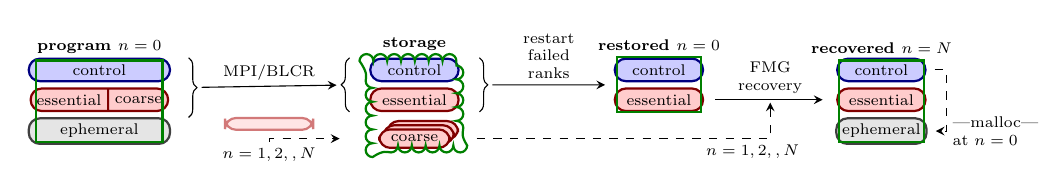
\begin{tikzpicture}
    [scale=0.8,every node/.style={scale=0.8},
    >=stealth,
    control/.style={rectangle,rounded corners,draw=blue!50!black,fill=blue!20,thick,minimum width=5em},
    essential/.style={rectangle,rounded corners,draw=red!50!black,fill=red!20,thick,minimum width=5em},
    ephemeral/.style={rectangle,rounded corners,draw=gray!50!black,fill=gray!20,thick,minimum width=5em},
    statebox/.style={rectangle,draw=green!50!black,thick},
    statetitle/.style={rectangle,draw=green!50!black,fill=green!20,thick},
    storebox/.style={rectangle,draw=},
    rightbrace/.style={decorate,decoration={brace,amplitude=1ex,raise=4pt}},
    leftbrace/.style={decorate,decoration={brace,amplitude=1ex,raise=4pt,mirror}}
    ]
    \scriptsize
    \node[control,minimum width=8em] (progcontrol) {control};
    \node[essential,below=2pt of progcontrol.south,rectangle split,rectangle split parts=2,rectangle split horizontal,minimum width=12em] (progessential) {essential \nodepart{two} coarse};
    \node[ephemeral,minimum width=8em,below=2pt of progessential.south] (progephemeral) {ephemeral};
    \node[statebox,fit=(progcontrol)(progessential)(progephemeral)] (progbox) {};
    \node[above=0pt of progbox.north,anchor=south] {\textbf{program $n=0$}};

    \node[control,right=9em of progcontrol] (storecontrol) {control};
    \node[essential,below=2pt of storecontrol.south] (storeessential) {essential};
    \node[essential,minimum width=4em,below=6pt of storeessential.south, double copy shadow] (storecoarse) {coarse};
    \node[statebox,decorate,decoration={bumps,mirror},fit=(storecontrol)(storecoarse)] (storebox) {};
    \node[above=1pt of storebox.north,anchor=south] {\textbf{storage}};

    \node[control,right=7em of storecontrol] (reccontrol) {control};
    \node[essential,below=2pt of reccontrol.south] (recessential) {essential};
    \node[statebox,fit=(reccontrol)(recessential)] (recbox) {};
    \node[above=0pt of recbox.north,anchor=south] {\textbf{restored $n=0$}};

    \node[control,right=6em of reccontrol] (donecontrol) {control};
    \node[essential,below=2pt of donecontrol.south] (doneessential) {essential};
    \node[ephemeral,below=2pt of doneessential.south] (doneephemeral) {ephemeral};
    \node[statebox,fit=(donecontrol)(doneephemeral)] (donebox) {};
    \node[above=0pt of donebox.north,anchor=south] {\textbf{recovered $n=N$}};

    \draw[decorate,decoration={brace,amplitude=1ex,raise=4pt}] ($(progcontrol.north east) + (3pt,0)$) -- ($(progephemeral.north east) + (3pt,0)$) node[midway,xshift=1ex] (progbrace) {};
    \draw[leftbrace] ($(storecontrol.north west) - (4pt,0)$) -- ($(storeessential.south west) - (4pt,0)$) node[midway,xshift=-1ex] (storebrace) {};
    \draw[rightbrace] ($(storecontrol.north east) + (4pt,0)$) -- ($(storeessential.south east) + (4pt,0)$) node[midway,xshift=1ex] (storerbrace) {};
    \draw[->,shorten >=4pt,shorten <=4pt] (progbrace) -- (storebrace) node[midway,above] (midarrow) {MPI/BLCR};

    \node[below=1.4em of midarrow,essential,draw=red!50!gray!70,fill=red!10] (coarserun) {};
    \draw[->,dashed,shorten >=14pt,shorten <=4pt] (coarserun) |- (storecoarse) node [near start,below,yshift=-3pt] {\scriptsize $n=1,2,\dotsc,N$};
    \draw[->,shorten >=4pt,shorten <=4pt] (storerbrace) -- (recbox.west) node[midway,above,text width=5em,align=center] (midarrow) {restart failed ranks};
    \draw[->,shorten >=5pt,shorten <=4pt] (recessential.east) -- (doneessential) node[midway,above,text width=5em,align=center] (fmgrecover) {FMG recovery};
    \draw[->,dashed,shorten >=1pt,shorten <=3pt] ($(storecoarse.east) + (1em,0)$) -| (fmgrecover) node[midway,below,xshift=-1em] {\scriptsize $n=1,2,\dotsc,N$};
    \draw[->,dashed,shorten >=3pt,shorten <=3pt] (donecontrol.east) -| ($(donecontrol.east) + (3ex,0)$) |- (doneephemeral.east) node[midway,right,text width=4em] {\cverb|malloc| at $n=0$};
  \end{tikzpicture}
\begin{description}
\item[control] contains program stack, solver configuration, etc.
\item[essential] program state that cannot be easily reconstructed: time-dependent solution, current optimization/bifurcation iterate
\item[ephemeral] easily recovered structures: assembled matrices, preconditioners, residuals, Runge-Kutta stage solutions
\end{description}
\begin{itemize}
\item Essential state at time/optimization step $n$ is \alert{inherently globally coupled} to step $n-1$ (otherwise we could use an explicit method)
\item \emph{Coarse} level checkpoints are orders of magnitude smaller, but allow rapid recovery of essential state
\item FMG recovery needs only \alert{nearest neighbors}
\end{itemize}
\end{frame}

\begin{frame}[fragile]{Multiscale compression and recovery using $\tau$ form}
   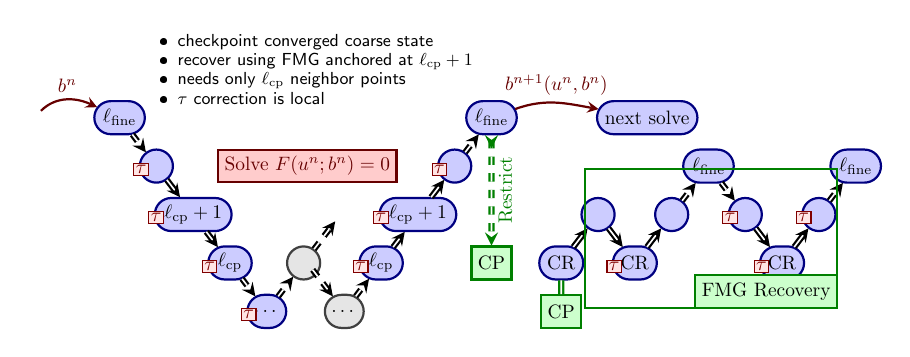
\begin{tikzpicture}
    [scale=0.7,every node/.style={scale=0.7},
    >=stealth,
    restrict/.style={thick,double},
    prolong/.style={thick,double},
    cprestrict/.style={green!50!black,thick,double,dashed},
    control/.style={rectangle,red!40!black,draw=red!40!black,thick},
    mglevel/.style={rounded rectangle,draw=blue!50!black,fill=blue!20,thick,minimum size=6mm},
    checkpoint/.style={rectangle,draw=green!50!black,fill=green!20,thick,minimum size=6mm},
    mglevelhide/.style={rounded rectangle,draw=gray!50!black,fill=gray!20,thick,minimum size=6mm},
    tau/.style={text=red!50!black,draw=red!50!black,fill=red!10,inner sep=1pt},
    crelax/.style={text=green!50!black,fill=green!10,inner sep=0pt}
    ]
    \begin{scope}
      \newcommand\mgdx{1.9em}
      \newcommand\mgdy{2.5em}
      \newcommand\mgloc[4]{(#1 + #4*\mgdx*#3,#2 + \mgdy*#3)}
      \node[mglevel] (fine0) at \mgloc{0}{0}{4}{-1} {\mglevelfine};
      \node[mglevel] (finem1down0) at \mgloc{0}{0}{3}{-1} {};
      \node[mglevel] (cp1down0) at \mgloc{0}{0}{2}{-1} {$\mglevelcp+1$};
      \node[mglevel] (cpdown0) at \mgloc{0}{0}{1}{-1} {\mglevelcp};
      \node[mglevel] (coarser0) at \mgloc{0}{0}{0}{0} {\ldots};

      \node[mglevelhide] (cpup0) at \mgloc{0}{0}{1}{1} {};
      \node (cp1up0) at \mgloc{0}{0}{2}{1} {};

      \node (cpdown1) at \mgloc{4em}{0}{1}{-1} {};
      \node[mglevelhide] (coarser1) at \mgloc{4em}{0}{0}{1} {\ldots};
      \node[mglevel] (cpup1) at \mgloc{4em}{0}{1}{1} {\mglevelcp};
      \node[mglevel] (cp1up1) at \mgloc{4em}{0}{2}{1} {$\mglevelcp+1$};
      \node[mglevel] (finem1up1) at \mgloc{4em}{0}{3}{1} {};
      \node[mglevel] (fine1) at \mgloc{4em}{0}{4}{1} {\mglevelfine};

      \draw[->,restrict,dashed] (fine0) -- (finem1down0);
      \draw[->,restrict] (finem1down0) -- (cp1down0);
      \draw[->,restrict] (cp1down0) -- (cpdown0);
      \draw[->,restrict,dashed] (cpdown0) -- (coarser0);
      \draw[->,prolong,dashed] (coarser0) -- (cpup0);
      \draw[->,prolong,dashed] (cpup0) -- (cp1up0);

      \draw[->,restrict,dashed] (cpdown1) -- (coarser1);
      \draw[->,prolong,dashed] (coarser1) -- (cpup1);
      \draw[->,prolong] (cpup1) -- (cp1up1);
      \draw[->,prolong] (cp1up1) -- (finem1up1);
      \draw[->,prolong,dashed] (finem1up1) -- (fine1);

      \node[checkpoint] at (4em + \mgdx*4,\mgdy) (cp) {CP};
      \draw[>->,cprestrict] (fine1) -- node[below,sloped] {Restrict} (cp);

      \node[left=\mgdx of fine0] (bnanchor) {};
      \node[control,fill=red!20] at (1.1*\mgdx,3*\mgdy) {Solve $F(u^n;b^n) = 0$};
      \node[mglevel,right=of fine1] (finedt) {next solve};
      \draw[->, >=stealth, control] (fine1) to[out=20,in=170] node[above] {$b^{n+1}(u^n,b^n)$} (finedt);
      \draw[->, >=stealth, control] (bnanchor) to[out=45,in=155] node[above] {$b^n$} (fine0);

      % Recovery process
      \begin{scope}[xshift=8*\mgdx]
        \node[checkpoint] (rcp) at \mgloc{0}{0}{0}{0} {CP};
        \node[mglevel] (r0a) at \mgloc{0}{\mgdy}{0}{0} {CR};
        \node[mglevel] (r1a) at \mgloc{0}{\mgdy}{1}{1} {};
        \node[mglevel] (r0b) at \mgloc{2*\mgdx}{\mgdy}{0}{0} {CR};
        \node[mglevel] (r1b) at \mgloc{2*\mgdx}{\mgdy}{1}{1} {};
        \node[mglevel] (r2b) at \mgloc{2*\mgdx}{\mgdy}{2}{1} {\mglevelfine};
        \node[mglevel] (r1c) at \mgloc{6*\mgdx}{\mgdy}{1}{-1} {};
        \node[mglevel] (r0d) at \mgloc{6*\mgdx}{\mgdy}{0}{0} {CR};
        \node[mglevel] (r1d) at \mgloc{6*\mgdx}{\mgdy}{1}{1} {};
        \node[mglevel] (r2d) at \mgloc{6*\mgdx}{\mgdy}{2}{1} {\mglevelfine};

        \draw[-,prolong,green!50!black] (rcp) -- (r0a);
        \draw[->,prolong] (r0a) -- (r1a);
        \draw[->,restrict] (r1a) -- (r0b);
        \draw[->,restrict] (r0b) -- (r1b);
        \draw[->,restrict,dashed] (r1b) -- (r2b);
        \draw[->,restrict,dashed] (r2b) -- (r1c);
        \draw[->,restrict] (r1c) -- (r0d);
        \draw[->,restrict] (r0d) -- (r1d);
        \draw[->,restrict,dashed] (r1d) -- (r2d);

        \foreach \smooth in {finem1down0, cp1down0, cpdown0, coarser0,
          cpup1, cp1up1, finem1up1,
          r0b,r1c,r0d,r1d} {
          \node[above left=-5pt of \smooth.west,tau] {$\tau$};
        }
        \node[rectangle,fill=none,draw=green!50!black,thick,fit=(rcp)(r2d)] (recoverbox) {};
        \node[rectangle,draw=green!50!black,fill=green!20,thick,minimum size=6mm,above={0cm of recoverbox.south east},anchor=south east] (recover) {FMG Recovery};
      \end{scope}
      \node (notation) at (\mgdx,5*\mgdy) {
        \begin{minipage}{18em}\small\sf
          \begin{itemize}\addtolength{\itemsep}{-5pt}
          \item checkpoint converged coarse state
          \item recover using FMG anchored at $\mglevelcp+1$
          \item needs only $\mglevelcp$ neighbor points
          \item $\tau$ correction is local
          \end{itemize}
        \end{minipage}
      };
    \end{scope}
  \end{tikzpicture}
  \begin{itemize}
  \item Normal multigrid cycles visit all levels moving from $n \to n+1$
  \item FMG recovery only accesses levels finer than $\ell_{CP}$
  \item Only failed processes and neighbors participate in recovery
  \item Lightweight checkpointing for transient adjoint computation
  \item Postprocessing applications, e.g., in-situ visualization at high temporal resolution in part of the domain
  \end{itemize}
\end{frame}

\begin{frame}{First-order cost model for FAS resilience}
  Extend first-order locality-unaware model of Young (1974):
  \begin{description}
  \item[$\timeW$] time to write a heavy fine-grid checkpointed state
  \item[$\timeR$] time to read back lost state
  \item[$R$] fraction of forward simulation needed for recomputation from a saved state
  \item[$P$] the heavy checkpoint interval
  \item[$M$] mean time to failure
  \end{description}
  Neglect cost of I/O for lightweight coarse-grid checkpoints
  \begin{equation*}\label{eq:overhead}
    \text{Overhead} = 1 - \text{AppUtilization} = \underbrace{\frac{\timeW}{P}}_{\text{writing}}
    + \underbrace{\frac{\timeR}{M}}_{\text{reading after failure}}
    + \underbrace{\frac{R P}{2M}}_{\text{recomputation}}
  \end{equation*}
  Minimized for a heavy checkpointing interval $P = \sqrt{2 M \timeW / R}$
  \begin{equation*}\label{eq:minoverhead}
    \text{Overhead}^* = \sqrt{2 \timeW R / M} + \timeR / M
    % $ \text{Overhead}^* = \sqrt{\frac{2 \timeW R}{M}} + \frac{\timeR}{M} $,
  \end{equation*}
  where the first term is always larger than the second.
  Conventional checkpointing schemes store only fine-grid state, thus $R=1$ (recovery costs the same as initial computation).
\end{frame}

\begin{frame}[fragile]
  \frametitle{Redundant Coarse-Grid Error Detection}
  A redundant coarse problem may be used to trivially check for errors:
  \begin{figure}
    \centering
    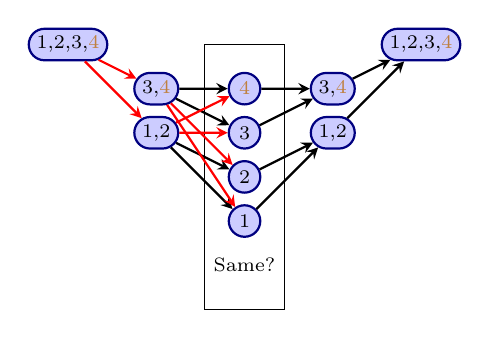
\begin{tikzpicture}
      [>=stealth,
      every node/.style={inner sep=2pt},
      restrict/.style={thick},
      prolong/.style={thick},
      mglevel/.style={rounded rectangle,draw=blue!50!black,fill=blue!20,thick,minimum size=4mm},
      ]
      \begin{scope}\scriptsize
        \newcommand\mgdx{4.0em}
        \newcommand\mgdy{4.0em}
        \newcommand\mgl[1]{(pow(2,#1+1))}
        \newcommand\mgloc[4]{(#1 + #4*\mgdx*#3,#2 + \mgdy*#3)}
        \node[mglevel] (down0) at \mgloc{0}{0}{2}{-1} {\red{1},\green{2},\blue{3},\color{brown}{4}};

        \node[mglevel] (down10) at \mgloc{0}{0}{1}{-1} {\red{1},\green{2}};
        \node[mglevel] (down11) at \mgloc{0}{0.5*\mgdy}{1}{-1} {\blue{3},\color{brown}{4}};

        \node[mglevel] (coarse0) at \mgloc{0}{0}{0}{-1} {\red{1}};
        \node[mglevel] (coarse1) at \mgloc{0}{0.5*\mgdy}{0}{-1} {\green{2}};
        \node[mglevel] (coarse2) at \mgloc{0}{1.0*\mgdy}{0}{-1} {\blue{3}};
        \node[mglevel] (coarse3) at \mgloc{0}{1.5*\mgdy}{0}{-1} {\color{brown}{4}};

        \node[] (same) at \mgloc{0}{-0.5*\mgdy}{0}{-1} {Same?};

        \draw \mgloc{-0.45*\mgdx}{-1.0*\mgdy}{0}{0} rectangle \mgloc{0.45*\mgdx}{2.0*\mgdy}{0}{0};

        \node[mglevel] (up10) at \mgloc{0}{0}{1}{1} {\red{1},\green{2}};
        \node[mglevel] (up11) at \mgloc{0}{0.5*\mgdy}{1}{1} {\blue{3},\color{brown}{4}};

        \node[mglevel] (up0) at \mgloc{0}{0}{2}{1} {\red{1},\green{2},\blue{3},\color{brown}{4}};

        \draw[->,restrict,red] (down0) -- (down10);
        \draw[->,restrict,red] (down0) -- (down11);

        \draw[->,restrict] (down10) -- (coarse0);
        \draw[->,restrict] (down10) -- (coarse1);

        \draw[->,restrict] (down11) -- (coarse2);
        \draw[->,restrict] (down11) -- (coarse3);

        % comm
        \draw[->,restrict,red] (down11) -- (coarse0);
        \draw[->,restrict,red] (down11) -- (coarse1);
        \draw[->,restrict,red] (down10) -- (coarse2);
        \draw[->,restrict,red] (down10) -- (coarse3);

        \draw[->,restrict] (coarse0) -- (up10);
        \draw[->,restrict] (coarse1) -- (up10);
        \draw[->,restrict] (coarse2) -- (up11);
        \draw[->,restrict] (coarse3) -- (up11);

        \draw[->,restrict] (up10) -- (up0);
        \draw[->,restrict] (up11) -- (up0);

      \end{scope}
    \end{tikzpicture}
    \label{fig:RedundantMGTest}
  \end{figure}
  However, this is uninteresting and doesn't exploit the algorithm; can we do anything better?
\end{frame}

\begin{frame}[fragile]
  \frametitle{$\tau$-Correction Error Detection}
  \begin{block}{Recall}
      At convergence, $u^{H*} = \hat I_h^H u^{h*}$ solves the $\tau$-corrected coarse grid equation
    $N^H u^H = f^H + \tau_h^H$,
    thus $\tau_h^H$ is the ``fine grid feedback'' that makes the coarse grid equation accurate.
  \end{block}
  \begin{figure}
    \centering
  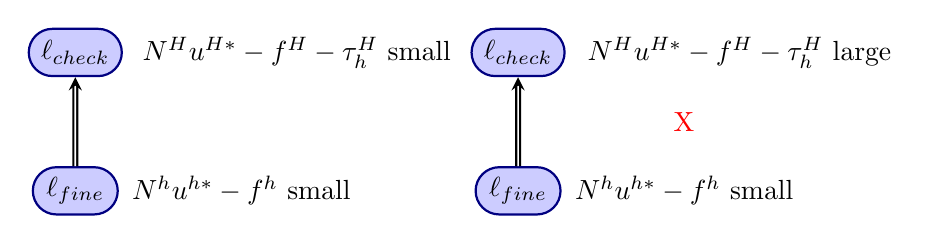
\begin{tikzpicture}
    [>=stealth,
    restrict/.style={thick,double},
    prolong/.style={thick,double},
    cprestrict/.style={green!50!black,thick,double,dashed},
    control/.style={rectangle,red!40!black,draw=red!40!black,thick},
    mglevel/.style={rounded rectangle,draw=blue!50!black,fill=blue!20,thick,minimum size=6mm},
    checkpoint/.style={rectangle,draw=green!50!black,fill=green!20,thick,minimum size=6mm},
    mglevelhide/.style={rounded rectangle,draw=gray!50!black,fill=gray!20,thick,minimum size=6mm},
    tau/.style={text=red!50!black,draw=red!50!black,fill=red!10,inner sep=1pt},
    crelax/.style={text=green!50!black,fill=green!10,inner sep=0pt}
    ]
    \newcommand\mgdx{2.0em}
    \newcommand\mgdy{2.5em}
    \newcommand\mgloc[4]{(#1 + #4*\mgdx*#3,#2 + \mgdy*#3)}
    \begin{scope}
      \node[mglevel] (fineright) at \mgloc{0}{0}{0}{0} {\mglevel$_{fine}$};
      \node[mglevel] (checkright) at \mgloc{0}{0}{2}{0} {\mglevel$_{check}$};
      \draw[->,restrict] (fineright) -- (checkright);

      \node[] (finerightnorm) at \mgloc{3*\mgdx}{0}{0}{0} {$\abs{N^h u^{h*} - f^h}$ small};
      \node[] (coarserightnorm) at \mgloc{4.0*\mgdx}{0}{2}{0} {$\abs{N^H u^{H*} - f^H - \tau_h^H}$ small};

      \node[mglevel] (finewrong) at \mgloc{8*\mgdx}{0}{0}{0} {\mglevel$_{fine}$};
      \node[mglevel] (checkwrong) at \mgloc{8*\mgdx}{0}{2}{0} {\mglevel$_{check}$};
      \draw[->,restrict] (finewrong) -- (checkwrong);

      \node[] (finewrongnorm) at \mgloc{11*\mgdx}{0}{0}{0} {$\abs{N^h u^{h*} - f^h}$ small};
      \node[] (coarsewrongnorm) at \mgloc{12.0*\mgdx}{0}{2}{0} {$\abs{N^H u^{H*} - f^H - \tau_h^H}$ large};

      \node[green] (OK) at \mgloc{3*\mgdx}{0}{1}{0} {\checkmark};
      \node[red] (BAD) at \mgloc{11*\mgdx}{0}{1}{0} {X};

    \end{scope}
  \end{tikzpicture}
  \end{figure}
  \begin{itemize}
  \item \emph{Local} detection if $\abs{N^H u^{H*} - f^H - \tau_h^H}$ is large
  \item incorrect result indicates error in fine grid residual evaluation (likely), restriction, or coarse grid residual.
  \end{itemize}
\end{frame}

\begin{frame}{Outlook on $\tau$-FAS}
  \begin{itemize}
  \item Nonlinear multigrid methods are more intrusive
  \item $\tau$-FAS is more sensitive to coarsening quality
  \item Ephemeral data is probably out of reach for most applications
  \item At Exascale, all stiff applications need multigrid
  \item Solver-friendly discretizations and user-friendly multigrid
  \item Identify reusable components suitable for architecture/discretization
  \item More emphasis on multiscale models
  \end{itemize}
\end{frame}

\begin{comment}
\section{Time Integration and nonlinear solvers}
\begin{frame}{Trade-offs in time integration}
  \begin{itemize}
  \item Properties
    \begin{itemize}
    \item Nonlinear stability (e.g., positivity preservation)
    \item Stability along imaginary axis
    \item $L$-stability (damping at infinity)
    \item Implicitness and reuse
    \end{itemize}
  \item What is expensive?
    \begin{itemize}
    \item Function evaluation
    \item Operator assembly/preconditioner setup
      \begin{itemize}
      \item How much can be reused for how long?
      \end{itemize}
    \item Implicit solves
      \begin{itemize}
      \item Can we find better solver algorithm?
      \item More effort in setup?
      \end{itemize}
    \end{itemize}
  \item What is ``convergence''?
    \begin{itemize}
    \item Wave propagation: implicitness useless for convergence \emph{in a norm}
    \item Non-norm functionals could be robust
    \end{itemize}
  \end{itemize}
\end{frame}

\begin{frame}{Reusing implicit solver setup}
  \begin{itemize}
  \item Linearization
  \item MG interpolants
  \item Lagged preconditioner
  \item Modified Newton
  \item Quasi-Newton
  \item IMEX with linear implicit part
  \item Rosenbrock/W
  \end{itemize}
\end{frame}

\begin{frame}[shrink=5]{IMEX time integration in PETSc}
  \begin{itemize}
  \item Additive Runge-Kutta IMEX methods
    \begin{gather*}
      G(t,x,\dot x) = F(t,x) \\
      J_\alpha = \alpha G_{\dot x} + G_x
    \end{gather*}
    \begin{itemize}
    \item User provides:
      \begin{itemize}
      \item \texttt{FormRHSFunction(ts,$t$,$x$,$F$,void *ctx);}
      \item \texttt{FormIFunction(ts,$t$,$x$,$\dot x$,$G$,void *ctx);}
      \item \texttt{FormIJacobian(ts,$t$,$x$,$\dot x$,$\alpha$,$J$,$J_{p}$,mstr,void *ctx);}
      \end{itemize}
    \item L-stable DIRK for stiff part $G$
    \item Choice of explicit method, \eg SSP
    \item Orders 2 through 5, embedded error estimates
    \item Dense output, hot starts for Newton
    \item More accurate methods if $G$ is linear, also Rosenbrock-W
    \item Can use preconditioner from classical ``semi-implicit'' methods
    \item Extensible adaptive controllers, can change order within a family
    \item Easy to register new methods: \code{TSARKIMEXRegister()}
    \end{itemize}
  \item Eliminate many interface quirks
  \item Single step interface so user can have own time loop
  \end{itemize}
\end{frame}


\begin{frame}[fragile]{Time integration method design}
  \begin{figure}
    \centering
    \includegraphics[width=.8\textwidth]{figures/TS/EmilMethodDesignFeatures.png}
  \end{figure}
  \begin{itemize}
  \item Select order, number of stages, required properties
  \item Optimize properties like SSP coefficient, accuracy, or linear stability
  \item \cverb|TSARKIMEXRegister("my-method", ...coefficients...)|
  \item \cverb|-ts_type arkimex -ts_arkimex_type my-method|
  \end{itemize}
\end{frame}

\begin{frame}{Example: Additive Runge-Kutta design}
  \begin{itemize}
  \item 3-stage, second order, $L$-stable implicit part
  \item one-parameter family of solutions
  \end{itemize}
  \begin{description}
  \item[ARK2c] Maximize SSP coefficient
  \item[ARK2E] Minimize leading error coefficient
  \end{description}
  \begin{figure}
    \centering
    \includegraphics[width=0.55\textwidth]{figures/TS/ssp_ark_poster.png}
    \includegraphics[width=0.49\textwidth]{figures/TS/Stability_ARK2E_ARK2C.pdf}
  \end{figure}
\end{frame}

\begin{frame}{Some TS methods}
  \begin{description}
  \item[TSSSPRK104] 10-stage, fourth order, low-storage, optimal explicit SSP Runge-Kutta $c_{\text{eff}} = 0.6$ (Ketcheson 2008)
  \item[TSARKIMEX2E] second order, one explicit and two implicit stages, $L$-stable, optimal (Constantinescu)
  \item[TSARKIMEX3] (and 4 and 5), $L$-stable (Kennedy and Carpenter, 2003)
  \item[TSROSWRA3PW] three stage, third order, for index-1 PDAE, $A$-stable, $R(\infty) = 0.73$, second order strongly $A$-stable embedded method (Rang and Angermann, 2005)
  \item[TSROSWRA34PW2] four stage, third order, $L$-stable, for index 1 PDAE, second order strongly $A$-stable embedded method (Rang and Angermann, 2005)
  \item[TSROSWLLSSP3P4S2C] four stage, third order, $L$-stable implicit, SSP explicit, $L$-stable embedded method (Constantinescu)
  \end{description}
\end{frame}


\begin{frame}{Adaptive controllers}
  \begin{itemize}
  \item ``Stiff'' waves are not stiff if one wants to converge \emph{in a norm}
    \begin{itemize}
    \item Implicit solve is a sort of filter
    \item MHD has many waves, speeds can be degenerate
    \end{itemize}
  \item Multiscale time integrators (HMM, FLAVORS) only converge in coarse variables
  \item PETSc integrators provide embedded methods to estimate errors
  \item Automatic controllers optimize local truncation error and nonlinear solve cost
  \item User can register custom controllers
  \item Use a priori knowledge of the physics, robust functionals
  \item Choose from list of methods, choose next step size
  \end{itemize}
\end{frame}

\begin{frame}{Nonlinear methods}
  \begin{itemize}
  \item Global linearization (NewtonLS, NewtonTR)
    \begin{itemize}
    \item Preconditioning libraries for assembled matrices, amortize setup cost
    \item Low arithmetic intensity
    \end{itemize}
  \item Quasi-Newton
    \begin{itemize}
    \item Build low-rank updates to Jacobian inverse
    \item B. and Brune, ``Low-rank quasi-Newton updates for robust Jacobian lagging in Newton-type methods'', ANS MC13.
    \end{itemize}
  \item Nonlinear multigrid and domain decomposition
    \begin{itemize}
    \item ASPIN (left-preconditioned nonlinear Schwarz), also right-preconditioned
    \item Full Approximation Scheme with linear or nonlinear smoothers
    \item More intrusive, but freakishly efficient for difficult problems
    \end{itemize}
  \item Nonlinear GMRES, Anderson mixing, nonlinear CG
    \begin{itemize}
    \item Accelerator for nonlinear preconditioning
    \item Good alternative to matrix-free finite differencing
    \item More robust line search possible: operates in reduced basis
    \end{itemize}
  \end{itemize}
\end{frame}

\begin{frame}
  \includegraphics[width=\textwidth]{figures/BruneNGMRESFAS2.png}
\end{frame}
\end{comment}

% \begin{frame}{The Great Solver Schism: Monolithic or Split?}
  \begin{columns}
    \begin{column}{0.5\textwidth}
      \begin{block}{Monolithic}
        \begin{itemize}
        \item Direct solvers
        \item Coupled Schwarz
        \item Coupled Neumann-Neumann \\
          (need unassembled matrices)
        \item Coupled multigrid
        \item[X] Need to understand local spectral and compatibility properties of the coupled system
        \end{itemize}
      \end{block}
    \end{column}
    \begin{column}{0.5\textwidth}
      \begin{block}{Split}
        \begin{itemize}
        \item Physics-split Schwarz \\
          (based on relaxation)
        \item Physics-split Schur \\
          (based on factorization)
          \begin{itemize}
          \item  approximate commutators \\
            SIMPLE, PCD, LSC
          \item segregated smoothers
          \item Augmented Lagrangian
          \item ``parabolization'' for stiff waves
          \end{itemize}
        \item[X] Need to understand global coupling strengths
        \end{itemize}
      \end{block}
    \end{column}
  \end{columns}
  \begin{itemize}
  \item Preferred data structures depend on which method is used.
  \item Interplay with geometric multigrid.
  \end{itemize}
\end{frame}

% \begin{frame}{Multi-physics coupling in PETSc}
  \begin{columns}
    \begin{column}{0.5\textwidth}
      \tikzstyle{cloud} = [draw, ellipse,fill=red!20, node distance=3cm, minimum height=2em]
      \tikzstyle{block} = [rectangle, draw, fill=blue!20, text width=5em, text centered, rounded corners, minimum height=2em]
      \begin{tikzpicture}
        \node [cloud] (momentum) {Momentum};
        \node [cloud, right of=momentum] (pressure) {Pressure};
        \node<2-> [block, opacity=0.5, fit=(momentum)(pressure), text opacity=0.8] (stokes) {Stokes};
        \node<3-> [cloud, below=2em of momentum] (energy) {Energy};
        \node<3-> [cloud, below=2em of pressure] (geometry) {Geometry};
        \node<4-> [block, opacity=0.4, fit=(stokes)(momentum)(pressure)(energy)(geometry), text opacity=0.8, text height=4em] (ice) {Ice};
        \node<5-> [block, below=2em of ice, minimum width=16em] (bl) {{Boundary \nolinebreak Layer}};
        \node<5-> [block, below=2em of bl, minimum width=16em] (ocean) {Ocean};
        % ]
      \end{tikzpicture}
    \end{column}
    \begin{column}{0.5\textwidth}
      \begin{itemize}
      \item package each ``physics'' independently
      \item solve single-physics and coupled problems
      \item semi-implicit and fully implicit
      \item reuse residual and Jacobian evaluation unmodified
      \item direct solvers, fieldsplit inside multigrid, multigrid inside fieldsplit without recompilation
      \item use the best possible matrix format for each physics \\ (e.g. symmetric block size 3)
      \item matrix-free anywhere
      \item multiple levels of nesting
      \end{itemize}
    \end{column}
  \end{columns}
\end{frame}

% \begin{frame}{Splitting for Multiphysics}
  \begin{equation*}
    \begin{bmatrix}
      A & B \\ C & D
    \end{bmatrix}
    \begin{bmatrix}
      x \\ y
    \end{bmatrix}
    =
    \begin{bmatrix}
      f \\ g
    \end{bmatrix}
  \end{equation*}
  \begin{itemize}\item Relaxation:
    \code{-pc\_fieldsplit\_type [additive,multiplicative,symmetric\_multiplicative]}
    \begin{equation*}
      \begin{bmatrix}
        A & \\  & D
      \end{bmatrix}^{-1} \qquad 
      \begin{bmatrix}
        A & \\ C & D
      \end{bmatrix}^{-1} \qquad
      \begin{bmatrix}
        A & \\  & \bm 1
      \end{bmatrix}^{-1}
      \left(
        \bm 1 -
        \begin{bmatrix}
          A & B \\ & \bm 1
        \end{bmatrix}
        \begin{bmatrix}
          A & \\ C & D
        \end{bmatrix}^{-1}
      \right)
    \end{equation*}
    \begin{itemize}
    \item Gauss-Seidel inspired, works when fields are loosely coupled
    \end{itemize}
  \item Factorization: \code{-pc\_fieldsplit\_type schur}
    \begin{align*}
      \begin{bmatrix}
        A & B \\ & S
      \end{bmatrix}^{-1}
      \begin{bmatrix}
        1 & \\ CA^{-1} & 1
      \end{bmatrix}^{-1}, \qquad
      S = D - C A^{-1} B
    \end{align*}
    \begin{itemize}
    \item robust (exact factorization), can often drop lower block
    \item how to precondition $S$ which is usually dense?
      \begin{itemize}
      \item interpret as differential operators, use approximate commutators
      \end{itemize}
    \end{itemize}
  \end{itemize}
\end{frame}

% \begin{frame}
  \includegraphics[width=\textwidth]{figures/PETSc/LocalSpaces} \\[-.5em]
  Work in Split Local space, matrix data structures reside in any space.
\end{frame}


\begin{frame}\LARGE
  \begin{itemize}
  \item Maximize science per Watt
  \item Huge scope remains at problem formulation
  \item Raise level of abstraction at which a problem is formally specified
  \item Algorithmic optimality is crucial
  \end{itemize}
\end{frame}

\end{document}
